\chapter{METODOLOGÍA DE LA INVESTIGACIÓN}
\section{Diseño de la investigación}
En esta sección del documento se explicará cual es el diseño, el tipo y el enfoque del trabajo de
investigación, así como también la población y la muestra. 
%Para finalizar se explicará el
%proceso de aplicación de las redes neuronales convolucionales.
\subsection{Enfoque de la investigación}
El presente trabajo tendrá un enfoque cuantitativo ya que se busca diseñar y desarrollar instrumentos, en este caso modelos predictivos, para responder al problema estudiado a partir de medición de datos históricos en la plataforma Kickstarter con herramientas basadas en la estadística y matemáticas que puedan ser interpretadas por cualquier investigador. 

\subsection{Alcance de la investigación}
El alcance del presente trabajo será descriptivo ya que se recolectarán datos en un determinado rango de tiempo (desde 2009 hasta el presente año 2019) para describir el comportamiento de las campañas de proyectos tecnológicos en Kickstarter a partir de las características de sus variables y con ello, pronosticar su posible éxito o fracaso antes de finalizar la campaña con un nivel óptimo de precisión.

\subsection{Tipo de la investigación}
Para determinar el tipo de la investigación, primero es necesario definir el actual trabajo como Diseño Experimental ya que las variables que se tienen serán controladas, es decir, serán agregadas o quitadas en el o los modelos construidos en el experimento para analizar el impacto que este o estos tendrán en los resultados obtenidos. Dentro de esta categoría se clasifica como Diseño Experimental Puro ya que se busca medir la variable dependiente, en este caso Status (el estado actual del proyecto en Kickstarter) a partir de la manipulación de las demás variables independientes agregando o desagregándolas para comparar los rendimientos obtenidos de los instrumentos de medición y determinar cuáles de ellas finalmente serán tomadas en cuenta.

\subsection{Descripción del prototipo de investigación}
Teniendo como referencia y base principal el décimo antecedente explicado en el Capítulo II, la idea del prototipo final consistió en ensamblar las tres partes básicas de un proyecto: la primera consiste en el tratamiento de la metainformación (en la cual se realizarán, asimismo, tres experimentos independientes), el segundo, en el contenido visual y el último, el contenido textual respectivamente pero con el valor diferenciado de adaptar el modelo general de acuerdo a las variables y conjuntos de datos disponibles para el presente trabajo. Para ello, se representa cada una de las tres partes agrupadas en el marco de trabajo de la Figura \ref{1:fig}.


\section{Población y muestra}

\subsection{Población}
La población que será considerada para el presente trabajo será de 27,251 proyectos en Kickstarter de la categoría tecnología de todas las subcategorías entre los periodos 2009-2019, en su mayoría del territorio de los Estados Unidos de América.

\subsection{Muestra}
Debido a que se 214 imágenes del contenido visual no pudieron re-dimensionarse, así como 2 proyectos no contaban con descripciones en el contenido textual, se procedió a remover los 216 proyectos incompletos tanto en la metainformación como en las otras bases de datos, resultando finalmente en 27,035 registros en cada una de los tres conjuntos de datos. Sin embargo, la división en subconjuntos fue distinta en los tres casos y se dio de la siguiente manera:

\begin{itemize}
	\item Para la metainformación y el contenido textual, el conjunto de datos total de cada uno fue dividido en un subconjunto de entrenamiento (80\%) y uno de prueba (20\%) siguiendo las proporciones dadas en el octavo antecedente.
	\item Para el contenido visual, el conjunto de datos total fue dividido en tres subconjuntos: entrenamiento (80\%), validación (10\%) y prueba (10\%) siguiendo las proporciones dadas en el décimo antecedente.
\end{itemize}

 Nisi porta lorem mollis aliquam ut porttitor leo. Aenean pharetra magna ac placerat vestibulum. Est placerat in egestas erat imperdiet sed euismod. Velit euismod in pellentesque massa placerat. Enim praesent elementum facilisis leo vel fringilla. Ante in nibh mauris cursus mattis molestie a iaculis. Erat pellentesque adipiscing commodo elit at imperdiet dui accumsan sit. Porttitor lacus luctus accumsan tortor posuere ac ut. Tortor at auctor urna nunc id. A iaculis at erat pellentesque adipiscing commodo elit. La Figura \ref{fig1} y el Cuadro \ref{tab:widgets}

	\begin{figure}[h]
		\begin{center}
			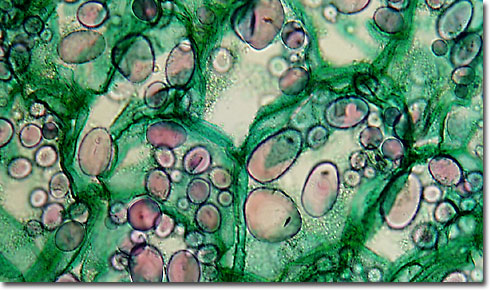
\includegraphics[width=0.8\textwidth]{3/figures/largepotato.jpg}
			\caption{Prueba de Figura}
			\label{fig1}
		\end{center}
		
	\end{figure}

\subsection{Unidad de análisis}
La unidad de análisis para el presente trabajo será un proyecto en Kickstarter de la categoría tecnología de cualquier subcategoría entre los periodos 2009-2019 dentro del territorio de los Estados Unidos de América.


\section{Operacionalización de Variables}

Nisi porta lorem mollis aliquam ut porttitor leo. Aenean pharetra magna ac placerat vestibulum. Est placerat in egestas erat imperdiet sed euismod. Velit euismod in pellentesque massa placerat. Enim praesent elementum facilisis leo vel fringilla. Ante in nibh mauris cursus mattis molestie a iaculis. Erat pellentesque adipiscing commodo elit at imperdiet dui accumsan sit. Porttitor lacus luctus accumsan tortor posuere ac ut. Tortor at auctor urna nunc id. A iaculis at erat pellentesque adipiscing commodo elit.
\section{Instrumentos de medida}
Nisi porta lorem mollis aliquam ut porttitor leo. Aenean pharetra magna ac placerat \begin{itemize}
	\item muscle and fat cells remove glucose from the blood,
	\item cells breakdown glucose via glycolysis and the citrate cycle, storing its energy in the form of ATP,
	\item liver and muscle store glucose as glycogen as a short-term energy reserve,
	\item adipose tissue stores glucose as fat for long-term energy reserve, and
	\item cells use glucose for protein synthesis.
\end{itemize}

\section{Técnicas de recolección de datos}
Nisi porta lorem mollis aliquam ut porttitor leo. Aenean pharetra magna ac placerat vestibulum. Est placerat in egestas erat imperdiet sed euismod. Velit euismod in pellentesque massa placerat. Enim praesent elementum facilisis leo vel fringilla. Ante in nibh mauris cursus mattis molestie a iaculis. Erat pellentesque adipiscing commodo elit at imperdiet dui accumsan sit. Porttitor lacus luctus accumsan tortor posuere ac ut. Tortor at auctor urna nunc id. A iaculis at erat pellentesque adipiscing commodo elit.

\LaTeX{} is great at typesetting mathematics. Let $X_1, X_2, \ldots, X_n$ be a sequence of independent and identically distributed random variables with
\begin{equation}
	S_n = \frac{X_1 + X_2 + \cdots + X_n}{n}
	= \frac{1}{n}\sum_{i}^{n} X_i
	\label{eq1}
\end{equation}

La Ecuación \ref{eq1} denote their mean. Then as $n$ approaches infinity, the random variables $$\sqrt{n}(S_n - \mu)$$ converge in distribution to a normal $\mathcal{N}(0, \sigma^2)$.

\section{Técnicas para el procesamiento y análisis de la información}
Nisi porta lorem mollis aliquam ut porttitor leo. Aenean pharetra magna ac placerat vestibulum. Est placerat in egestas erat imperdiet sed euismod. Velit euismod in pellentesque massa placerat. Enim praesent elementum facilisis leo vel fringilla. Ante in nibh mauris cursus mattis molestie a iaculis. Erat pellentesque adipiscing commodo elit at imperdiet dui accumsan sit. Porttitor lacus luctus accumsan tortor posuere ac ut. Tortor at auctor urna nunc id. A iaculis at erat pellentesque adipiscing commodo elit.

You can make lists with automatic numbering \dots

\begin{enumerate}
	\item Like this,
	\item and like this.
\end{enumerate}
\dots or bullet points \dots
\begin{itemize}
	\item Like this,
	\item and like this.
\end{itemize}


\section{Cronograma de actividades y presupuesto}
Nisi porta lorem mollis aliquam ut porttitor leo. Aenean pharetra magna ac placerat vestibulum. Est placerat in egestas erat imperdiet sed euismod. Velit euismod in pellentesque massa placerat. Enim praesent elementum facilisis leo vel fringilla. Ante in nibh mauris cursus mattis molestie a iaculis. Erat pellentesque adipiscing commodo elit at imperdiet dui accumsan sit. Porttitor lacus luctus accumsan tortor posuere ac ut. Tortor at auctor urna nunc id. A iaculis at erat pellentesque adipiscing commodo elit.

\begin{table}[h]
	\centering
	\begin{tabular}{l|r}
		Item & Quantity \\\hline
		Widgets & 42 \\
		Gadgets & 13
	\end{tabular}
	\caption{\label{tab:widgets}An example table.}
\end{table}